\documentclass[10pt,a4paper,notitlepage]{article}
\usepackage[utf8]{inputenc}
\usepackage[polish]{babel}
\usepackage[T1]{fontenc}
\usepackage{fullpage}
\usepackage{amsmath}
\usepackage{graphicx}
%\usepackage{placeins}
\usepackage{multirow}
\usepackage[a4paper,margin=1in]{geometry}
\usepackage{lscape}
\usepackage{hyperref}

\setlength{\parindent}{4em}
\setlength{\parskip}{1em}
\renewcommand{\baselinestretch}{1.3}

\author{Radosław Błażewicz, Fatoumata Bocar}
\title{Dziennik szkolny - baza danych\\		
		\Large
		Dokumentacja projektu\\
		}
\date{Styczeń 2020}

\begin{document}
\maketitle

\tableofcontents

\section{Struktura bazy danych}


\subsection{Modele i diagramy}\hyperref[fig1]{Rys. 1} przedstawia diagram przypadków użycia. \hyperref[fig2]{Rys. 2} przedstawia model logiczny stworzonej bazy danych.



\subsection{Tabele}
Przetwarzane grupy danych zostały zdefiniowane w tabelach opisanych poniżej. Tabele Użytkownik i Modyfikacja oraz wszystkie powiązania z nimi zostały zaimplementowane dla ułatwienia zarządzania oraz zwiększenia bezpieczeństwa przetwarzanych informacji.


\subsubsection{Klasa}
Tabela ta zawiera podstawowe informacje dot. danej klasy. Pole ID\_wychowawcy odnosi się do klucza idNauczyciel tablicy Nauczyciel, wskazując na nauczyciela odpowiedzialnego na daną klasę.

Kolumny tabeli Klasa opisuje \hyperref[tab1]{Tabela 1}.



\subsubsection{Kontakt}
Tabela ta zawiera pojedyncze dane teleadresowe danej osoby. Pole ID\_osoby odnosi się do klucza idOsoba tablicy Osoba, wskazując na nauczyciela odpowiedzialnego na daną klasę. Pole ID\_rodzaju\_kontaktu odnosi się do klucza id\_Rodzaju\_Kontaktu tablicy Rodzaj\_Kontaku będącej słownikiem możliwych typów danych kontaktowych.

Kolumny tabeli Kontakt opisuje \hyperref[tab2]{Tabela 2}.


\subsubsection{Modyfikacja}
Tabela ta zawiera podstawowe informacje dot. ostatniej dokonanej modyfikacji rekordu. Pole id\\\_użytkownika odnosi się do klucza idUżytkownika tablicy Użytkownik i wskazuje na użytkownika, który dokonał modyfikacji.

Kolumny tabeli Modyfikacja opisuje \hyperref[tab3]{Tabela 3}.

\subsubsection{Nauczyciel}
Tabela ta wiążę daną osobę z rolą nauczyciela. Pole ID\_osoby odnosi się do klucza idOsoba tablicy Osoba i jest powiązaniem z danymi osobowymi nauczyciela.

Kolumny tabeli Nauczyciel opisuje \hyperref[tab4]{Tabela 4}.

\subsubsection{Nauczyciel\_przedmiot}
Tabela ta pozwala powiązać nauczycieli z prowadzonymi przedmiotami relacją wiele-do-wielu. Pole ID\_Nauczyciel odnosi się do klucza idNauczyciel tablicy Nauczyciel i jest powiązaniem z nauczycielem uczącym przedmiotu. Pole ID\_Przedmiot odnosi się do klucza idPrzedmiot tablicy Przedmiot i jest powiązaniem z uczonym przedmiotem.

Kolumny tabeli Nauczyciel opisuje \hyperref[tab5]{Tabela 5}.
\subsubsection{Obecność}
Tabela ta zawiera informacje o stanach obecności uczniów na danych przedmiotach. Pole ID\_Przedmiotu odnosi się do klucza idPrzedmiot tablicy Przedmiot i jest powiązaniem z przedmiotem na którym sprawdzana była obecność. Pole ID\_ucznia odnosi się do klucza idUczeń tablicy Uczeń i jest powiązaniem z uczniem którego dotyczy sprawdzona obecność. Pole ID\_nauczyciela odnosi się do klucza idNauczyciel tablicy Nauczyciel i jest powiązaniem z nauczycielem uczącym przedmiotu. 

Kolumny tabeli Obecność opisuje \hyperref[tab6]{Tabela 6}.
\subsubsection{Ocena}
Tabela ta zawiera informacje dot. wystawionych ocen. Pole ID\_Przedmiotu odnosi się do klucza idPrzedmiot tablicy Przedmiot i jest powiązaniem z przedmiotem na którym wystawiona została ocena. Pole ID\_rodzaju\_oceny odnosi się do klucza idRodzaju\_Oceny tablicy Rodzaj\_Oceny i informacją o cechach wystawionej oceny. Pole ID\_ucznia odnosi się do klucza idUczeń tablicy Uczeń i jest powiązaniem z uczniem którego dotyczy wystawiona ocena. Pole ID\_nauczyciela odnosi się do klucza idNauczyciel tablicy Nauczyciel i jest powiązaniem z nauczycielem, który wystawił ocenę. 

Kolumny tabeli Ocena opisuje \hyperref[tab7]{Tabela 7}.
\subsubsection{Osoba}
Tabela ta zawiera dane osobowe użytkowników bazy danych.

Kolumny tabeli Osoba opisuje \hyperref[tab8]{Tabela 8}.
\subsubsection{Przedmiot}
Tabela ta zawiera informacje o danym przedmiocie.
Pole ID\_Rodzaj\_Przedmiotu odnosi się do klucza idRodzaj\_Przedmiotu tablicy Rodzaj\_Przedmiotu i odnosi się do słownika charakterystyk przedmiotów. Pole ID\_klasy odnosi się do klucza idKlasa tablicy Klasa i odnosi się do klasy, w której prowadzony jest przedmiot.

Kolumny tabeli Przedmiot opisuje \hyperref[tab9]{Tabela 9}.
\subsubsection{Rodzaj\_kontaktu}
Tabela jest słownikiem typów danych kontaktowych.
Kolumny tabeli Rodzaj\_kontaktu opisuje \hyperref[tab10]{Tabela 10}.
\subsubsection{Rodzaj\_oceny}
Tabela jest słownikiem typów ocen oraz ich charakterystyk.
Kolumny tabeli Rodzaj\_oceny opisuje \hyperref[tab11]{Tabela 11}.
\subsubsection{Rodzaj\_przedmiotu}
Tabela jest słownikiem prowadzonych przedmiotów.
Kolumny tabeli Rodzaj\_przedmiotu opisuje \hyperref[tab12]{Tabela 12}.
\subsubsection{Rola\_użytkownika}
Tabela jest słownikiem ról użytkowników oraz ich uprawnień.
Kolumny tabeli Rola\_użytkownika opisuje \hyperref[tab13]{Tabela 13}.
\subsubsection{Średnia}
Tabela ta zawiera informacje dot. średnich ocen. Pole ID\_osoby odnosi się do klucza idOsoba tablicy osoba i stanowi powiązanie między średnią, a osobą dla której została obliczona. Pole ID\_przedmiotu stanowi powiązanie między średnią, a przedmiotem z którego została obliczona. Pole ID\_klasy stanowi powiązanie między średnią, a klasą dla której została obliczona.
Kolumny tabeli Średnia opisuje \hyperref[tab14]{Tabela 14}.
\subsection{Średnia\_Ocena}
\subsubsection{Uczeń}
Tabela ta zawiera informacje dotyczące uczniów. Pole ID\_osoby odnosi się do klucza idOsoba tablicy Osoba i jest powiązaniem między uczniem a jego danymi osobowymi. Pole ID\_klasy odnosi się do klucza idKlasa tablicy Klasa i jest równoznaczne z zapisaniem ucznia do danej klasy. Pole ID\_opiekuna odnosi się do klucza idOsoba tablicy Osoba i jest powiązaniem między uczniem a opiekunem.
Kolumny tabeli Uczeń opisuje \hyperref[tab15]{Tabela 15}.
\subsubsection{Uczeń\_opiekun}
Tablica ta jest tablicą pomocniczą, umożliwiającej połączenie uczniów z ich opiekunami relacją wiele-do-wielu.
Kolumny tabeli Uczeń\_opiekun opisuje \hyperref[tab16]{Tabela 16}.
\subsubsection{Uwagi\_szkolne}
Tablica ta przechowuje wystawione uwagi szkolne. Pole ID\_nauczyciela odnosi się do klucza idNauczyciel tablicy Nauczyciel i wskazuje na nauczyciela wystawiającego uwagę. Pole ID\_Ucznia odnosi się do klucza idUczeń tablicy Uczeń i wskazuje na ucznia, któremu wystawiana jest uwaga.
Kolumny tabeli Uwagi\_szkolne opisuje \hyperref[tab17]{Tabela 17}.
\subsubsection{Użytkownik}
Tablica ta jest zbiorem danych o kontach użytkowników. Pole ID\_osoby odnosi się do klucza idOsoba tablicy Osoba i jest powiązaniem między kontem użytkownika a jego danymi osobowymi. Pole id\_roli\_użytkownika odnosi się do klucza idRola\_użytkownika tablicy Rola\_użytkownika i wskazuje na informacje dot. praw dostępu.
Kolumny tabeli Użytkownik opisuje \hyperref[tab18]{Tabela 18}.
\subsection{Procedury i triggery}
\subsection{Widoki}
\subsection{Użytkownicy}

\section{Opis aplikacji zarządzającej}

\section{Rysunki i tabele}
\begin{figure}[p]
\label{fig1}
\centering
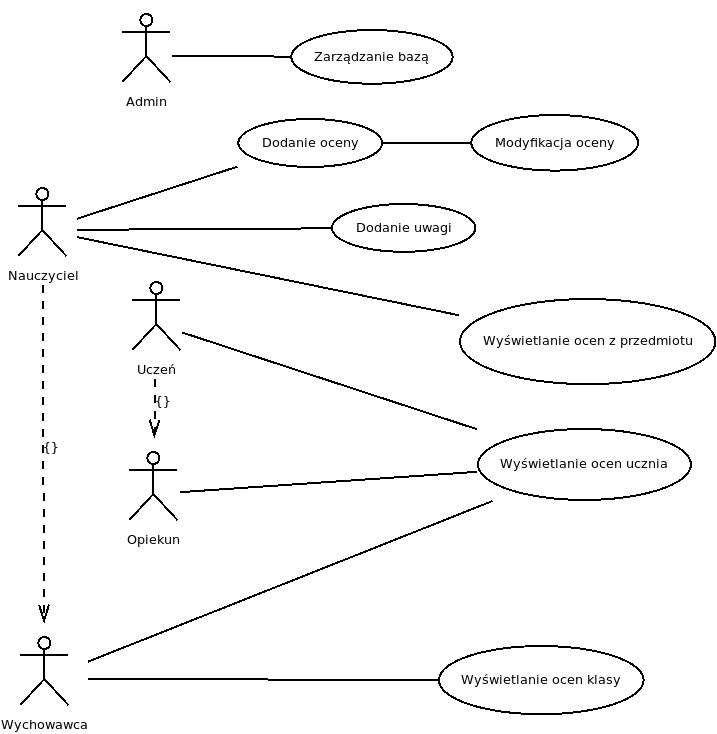
\includegraphics[width=0.55\textwidth]{diagram_uzycia.png}
\caption{Diagram przypadków użycia}
\end{figure}
\begin{landscape}

\begin{figure}[p]
\centering
\label{fig2}
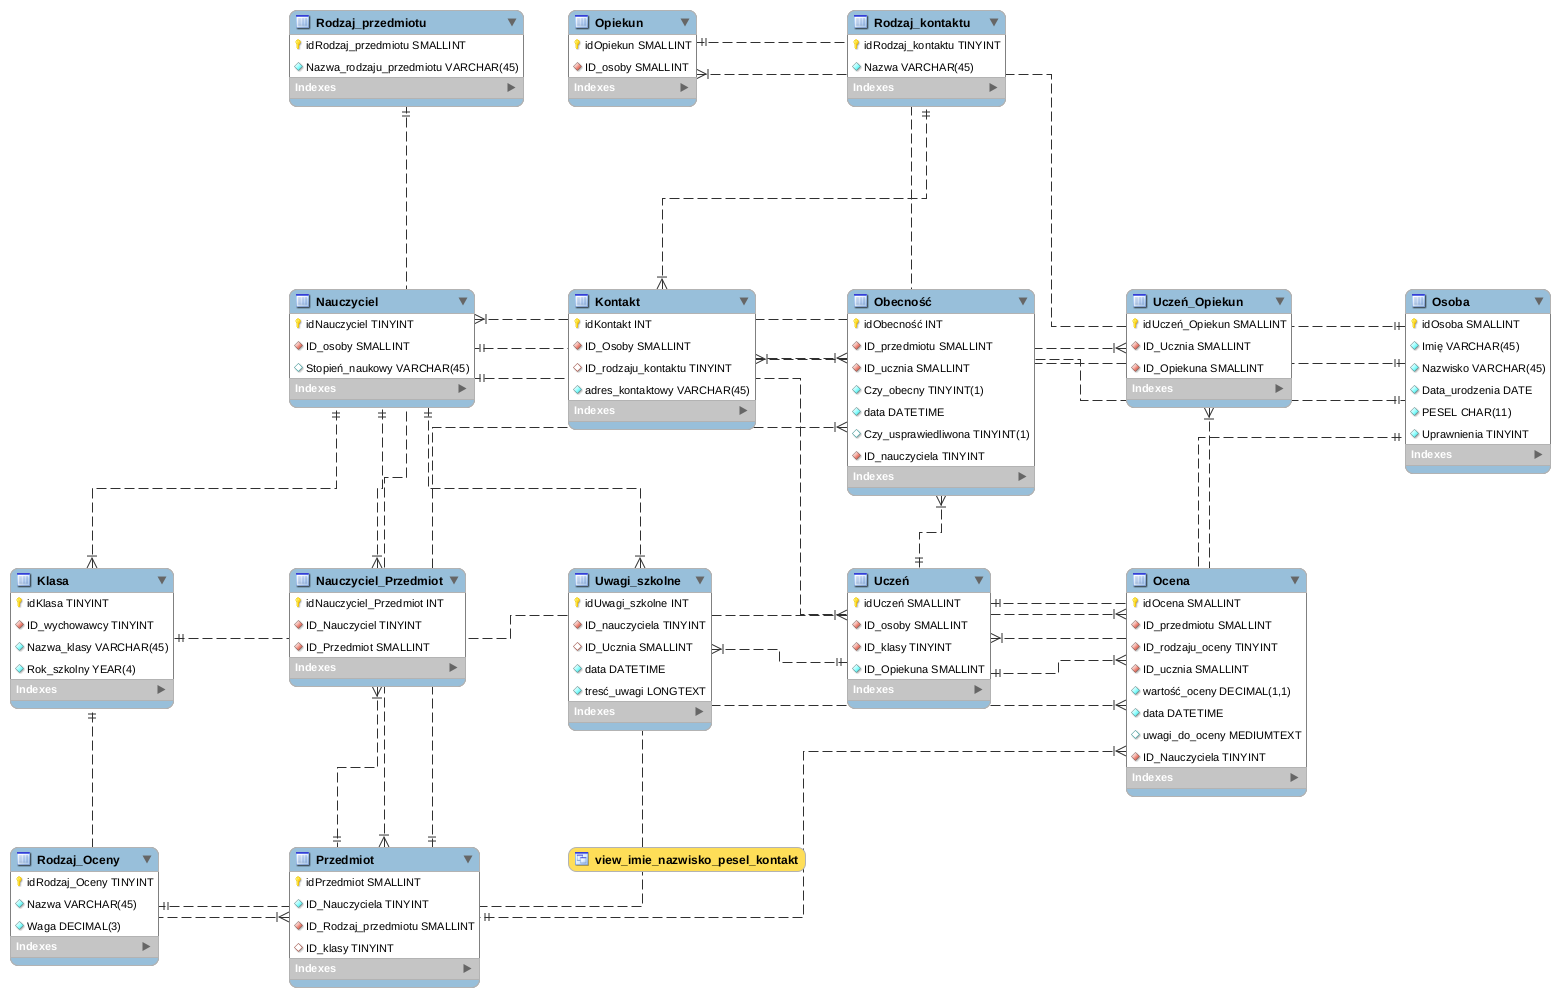
\includegraphics[width=1.25\textwidth]{model.png}
\caption{Model logiczny bazy danych}
\end{figure}


\begin{table}[p]
\label{tab1}
\begin{tabular}{|l|l|l|l|l|l|}
\hline
\textbf{Nazwa kolumny} & \textbf{Typ danych} & \textbf{Zakres wartości} & \textbf{Index} & \textbf{Przyjmuje Null} & \textbf{Opis}                  \\ \hline
idKlasa                & TINYINT             &                          &                & Nie                     & Identyfikator rekordu          \\ \hline
ID\_wychowawcy         & TINYINT             &                          &                & Nie                     & Identyfikator wychowawcy klasy \\ \hline
Nazwa\_klasy           & VARCHAR(45)         &                          &                & Nie                     & Numer bądź nazwa klasy         \\ \hline
Rok\_szkolny           & YEAR(4)             &                          &                & Nie                     & Rok utworzenia klasy           \\ \hline
idModyfikacji	& SMALLINT					&					&				& Nie						& Informacje dot. ostatniej modyfikacji rekordu
\\ \hline
\end{tabular}
\caption{Opis tabeli Klasa}
\end{table}

\begin{table}[p]
\label{tab2}
\begin{tabular}{|l|l|l|l|l|l|}
\hline
\textbf{Nazwa kolumny} & \textbf{Typ danych} & \textbf{Zakres wartości} & \textbf{Index} & \textbf{Przyjmuje Null} & \textbf{Opis}                                                           \\ \hline
idKontakt              & INT                 &                          &                & Nie                     & Identyfikator rekordu                                                   \\ \hline
ID\_Osoby              & SMALLINT            &                          &                & Nie                     & Identyfikator osoby powiązanej z danymi kontaktowymi                    \\ \hline
ID\_rodzaju\_kontaktu  & TINYINT             &                          &                & Tak                     & Identyfikator rodzaju przechowywanej inforamcji \\ \hline
adres\_kontaktowy      & VARCHAR(150)        &                          &                & Nie                     & Dane adresowe                                                           \\ \hline
\end{tabular}
\caption{Opis tabeli Kontakt}
\end{table}

\begin{table}[p]
\label{tab3}
\begin{tabular}{|l|l|l|l|l|l|}
\hline
\textbf{Nazwa kolumny} & \textbf{Typ danych} & \textbf{Zakres wartości} & \textbf{Index} & \textbf{Przyjmuje Null} & \textbf{Opis}                                         \\ \hline
idModyfikacja          & SMALLINT            &                          &                & Nie                     & Identyfikator rekordu                                 \\ \hline
data\_modyfikacji      & DATE                &                          &                & Nie                     & Data ostatniej dokonanej modyfikacji                  \\ \hline
id\_Użytkownika        & SMALLINT            &                          &                & Tak                     & Identyfikator użytkownika, który dokonał modyfikacji. \\ \hline

\end{tabular}
\caption{Opis tabeli Modyfikacja}
\end{table}

\begin{table}[p]
\label{tab4}
\begin{tabular}{|l|l|l|l|l|l|}
\hline
\textbf{Nazwa kolumny} & \textbf{Typ danych} & \textbf{Zakres wartości} & \textbf{Index} & \textbf{Przyjmuje Null} & \textbf{Opis}                                     \\ \hline
idNauczyciel           & TINYINT             &                          &                & Nie                     & Identyfikator rekordu                             \\ \hline
ID\_Osoby              & SMALLINT            &                          &                & Nie                     & Identyfikator osoby pełniącej funkcję nauczyciela \\ \hline
Stopień naukowy        & VARCHAR             &                          &                & Tak                     & Informacja dot. tytułu akademickiego nauczyciela  \\ \hline
\end{tabular}
\caption{Opis tabeli Nauczyciel}
\end{table}

\begin{table}[p]
\label{tab5}
\begin{tabular}{|l|l|l|l|l|l|}

\hline
\textbf{Nazwa kolumny}  & \textbf{Typ danych} & \textbf{Zakres wartości} & \textbf{Index} & \textbf{Przyjmuje Null} & \textbf{Opis}             \\ \hline
idNauczyciel\_Przedmiot & INT                 &                          &                & Nie                     & Identyfikator rekordu     \\ \hline
ID\_Nauczyciel          & TINYINT             &                          &                & Nie                     & Identyfikator nauczyciela \\ \hline
ID\_Przedmiot           & SMALLINT            &                          &                & Nie                     & Identyfikator przedmiotu  \\ \hline
\end{tabular}
\caption{Opis tabeli Nauczyciel\_Przedmiot}
\end{table}

\begin{table}[p]
\label{tab6}
\begin{tabular}{|l|l|l|l|l|l|}
\hline
\textbf{Nazwa kolumny} & \textbf{Typ danych} & \textbf{Zakres wartości} & \textbf{Index} & \textbf{Przyjmuje Null} & \textbf{Opis}                                     \\ \hline
idObecność             & INT                 &                          &                & Nie                     & Identyfikator rekordu                             \\ \hline
ID\_Przedmiotu         & SMALLINT            &                          &                & Nie                     & Identyfikator przedmiotu którego dotyczy obecność \\ \hline
ID\_ucznia             & SMALLINT            &                          &                & Nie                     & Identyfikator ucznia                              \\ \hline
Czy\_obecny            & TINYINT(1)          &                          &                & Nie                     & Pole informujące o stanie obecności ucznia        \\ \hline
data                   & DATETIME            &                          &                & Nie                     & Czas sprawdzania obecności                        \\ \hline
Czy\_usprawiedliwiona  & TINYINT(1)          &                          &                & Tak                     & Status ewentualnej nieobecności                   \\ \hline
ID\_nauczyciela        & TINYINT             &                          &                & Nie                     & Identyfikator nauczyciela sprawdzającego obecność \\ \hline
idModyfikacji          & SMALLINT            &                          &                & Nie                     & Identyfikator danych ostatniej modyfikacji        \\ \hline
\end{tabular}
\caption{Opis tabeli Modyfikacja}
\end{table}

\begin{table}[p]
\label{tab7}
\begin{tabular}{|l|l|l|l|l|l|}
\hline
\textbf{Nazwa kolumny} & \textbf{Typ danych} & \textbf{Zakres wartości} & \textbf{Index} & \textbf{Przyjmuje Null} & \textbf{Opis}                                       \\ \hline
idOcena                & SMALLINT            &                          &                & Nie                     & Identyfikator rekordu                               \\ \hline
ID\_przedmiotu         & SMALLINT            &                          &                & Nie                     & Identyfikator przedmiotu którego dotyczy ocena      \\ \hline
ID\_rodzaju\_oceny     & TINYINT             &                          &                & Nie                     & Identyfikator rodzaju wystawianej oceny             \\ \hline
ID\_ucznia             & SMALLINT            &                          &                & Nie                     & Identyfikator ucznia, któremu wystawiana jest ocena \\ \hline
wartość\_oceny         & DECIMAL(2,1)        &                          &                & Nie                     & -                                                   \\ \hline
data\_oceny            & DATETIME            &                          &                & Nie                     & Data wystawienia oceny                              \\ \hline
uwagi\_do\_oceny       & MEDIUMTEXT          &                          &                & Tak                     & -                                                   \\ \hline
ID\_nauczyciela        & TINYINT             &                          &                & Nie                     & Identyfikator nauczyciela wystawiającego ocenę      \\ \hline
idModyfikacji          & SMALLINT            &                          &                & Nie                     & Identyfikator danych ostatniej modyfikacji          \\ \hline
ID\_średnia\_ocena & SMALLINT & & Nie & Idenyfikator średniej
\end{tabular}
\caption{Opis tabeli Ocena}
\end{table}

\begin{table}[]
\label{tab8}
\begin{tabular}{|l|l|l|l|l|l|}
\hline
\textbf{Nazwa kolumny} & \textbf{Typ danych} & \textbf{Zakres wartości} & \textbf{Index} & \textbf{Przyjmuje Null} & \textbf{Opis}                                  \\ \hline
idOsoba                & SMALLINT            &                          &                & Nie                     & Identyfikator rekordu                          \\ \hline
Imię                   & VARCHAR(45)         &                          &                & Nie                     & -                                              \\ \hline
Nazwisko               & VARCHAR(45)         &                          &                & Nie                     & -                                              \\ \hline
Data\_urodzenia        & DATE                &                          &                & Nie                     & -                                              \\ \hline
PESEL                  & CHAR(11)            &                          &                & Nie                     & -                                              \\ \hline
idModyfikacji          & SMALLINT            & Nie                      &                & Nie                     & Identyfikator danych ostatniej modyfikacji     \\ \hline
\end{tabular}
\caption{Opis tabeli Osoba}
\end{table}

\begin{table}[p]
\label{tab9}
\begin{tabular}{|l|l|l|l|l|l|}
\hline
\textbf{Nazwa kolumny} & \textbf{Typ danych} & \textbf{Zakres wartości} & \textbf{Index} & \textbf{Przyjmuje Null} & \textbf{Opis}                                     \\ \hline
idPrzedmiot            & SMALLINT            &                          &                & Nie                     & Identyfikator rekordu                             \\ \hline
ID\_Rodzaj\_przedmiotu & SMALLINT            &                          &                & Nie                     & Identyfikator informacji o szczegółach przedmiotu \\ \hline
ID\_klasy              & TINYINT             &                          &                & Nie                     & Identyfikator klasy, która uczy się przedmiotu    \\ \hline
idModyfikacji          & SMALLINT            & Nie                      &                & Nie                     & Identyfikator danych ostatniej modyfikacji        \\ \hline
\end{tabular}
\caption{Opis tablicy Przedmiot}
\end{table}

\begin{table}[p]
\label{tab10}
\begin{tabular}{|l|l|l|l|l|l|}
\hline
\textbf{Nazwa kolumny} & \textbf{Typ danych} & \textbf{Zakres wartości} & \textbf{Index} & \textbf{Przyjmuje Null} & \textbf{Opis}                                  \\ \hline
idRodzaj\_kontaktu     & TINYINT             &                          &                & Nie                     & Identyfikator rekordu                          \\ \hline
Nazwa                  & VARCHAR(45)         &                          &                & Nie                     & Opis rodzaju kontaktu                          \\ \hline
idModyfikacji          & SMALLINT            &                          &                & Nie                     & Identyfikator danych ostatniej modyfikacji     \\ \hline
\end{tabular}
\caption{Opis tablicy Rodzaj\_kontaktu}
\end{table}

\begin{table}[p]
\label{tab11}
\begin{tabular}{|l|l|l|l|l|l|}
\hline
\textbf{Nazwa kolumny} & \textbf{Typ danych} & \textbf{Zakres wartości} & \textbf{Index} & \textbf{Przyjmuje Null} & \textbf{Opis}                                  \\ \hline
idRodzaj\_oceny        & TINYINT             &                          &                & Nie                     & Identyfikator rekordu                          \\ \hline
Nazwa                  & VARCHAR(45)         &                          &                & Nie                     & Opis rodzaju oceny                             \\ \hline
Waga                   & DECIMAL(3)          &                          &                & Nie                     & Waga oceny                                     \\ \hline
idModyfikacji          & SMALLINT            &                          &                & Nie                     & Identyfikator danych ostatniej modyfikacji     \\ \hline
\end{tabular}
\caption{Opis tablicy Rodzaj\_Oceny}
\end{table}

\begin{table}[p]
\label{tab12}
\begin{tabular}{|l|l|l|l|l|l|}
\hline
\textbf{Nazwa kolumny}     & \textbf{Typ danych} & \textbf{Zakres wartości} & \textbf{Index} & \textbf{Przyjmuje Null} & \textbf{Opis}                                  \\ \hline
idRodzaj\_oceny            & TINYINT             &                          &                & Nie                     & Identyfikator rekordu                          \\ \hline
Nazwa\_rodzaju\_przedmiotu & VARCHAR(45)         &                          &                & Nie                     & Opis rodzaju przedmiotu                        \\ \hline
idModyfikacji              & SMALLINT            &                          &                & Nie                     & Identyfikator danych ostatniej modyfikacji     \\ \hline
\end{tabular}
\caption{Opis tablicy Rodzaj\_przedmiotu}
\end{table}

\begin{table}[p]
\label{tab13}
\begin{tabular}{|l|l|l|l|l|l|}
\hline
\textbf{Nazwa kolumny}  & \textbf{Typ danych} & \textbf{Zakres wartości} & \textbf{Index} & \textbf{Przyjmuje Null} & \textbf{Opis}                                  \\ \hline
idRola\_użytkownika     & SMALLINT            &                          &                & Nie                     & Identyfikator rekordu                          \\ \hline
opis\_roli\_użytkownika & VARCHAR(45)         &                          &                & Nie                     & -                                              \\ \hline
idModyfikacji           & SMALLINT            &                          &                & Nie                     & Identyfikator danych ostatniej modyfikacji     \\ \hline
uprawnienia             & TINYINT             &                          &                & Nie                     & Poziom uprawnień użytkowników o danej roli     \\ \hline

\end{tabular}
\caption{Opis tablicy Rola\_użytkownika}
\end{table}

\begin{table}[p]
\label{tab14}
\begin{tabular}{|l|l|l|l|l|l|}
\hline
\textbf{Nazwa kolumny} & \textbf{Typ danych} & \textbf{Zakres wartości} & \textbf{Index} & \textbf{Przyjmuje Null} & \textbf{Opis}                                      \\ \hline
idŚrednia              & SMALLINT            &                          &                & Nie                     & Identyfikator rekordu                              \\ \hline
id\_osoby              & SMALLINT            &                          &                & Nie                     & Identyfikator danych osoby, której dotyczy średnia \\ \hline
id\_przedmiotu         & SMALLINT            &                          &                & Nie                     & Identyfikator przedmiotu, którego dotyczy średnia  \\ \hline
idModyfikacji          & SMALLINT            &                          &                & Nie                     & Identyfikator danych ostatniej modyfikacji         \\ \hline
id\_klasy              & SMALLINT            &                          &                & Nie                     & Identyfikator klasy, której dotyczy średnia         \\ \hline
wartość          & DECIMAL(3,2)         &                          &                & Nie                     & Wartość średniej ważonej z przedmiotu        \\ \hline
\end{tabular}
\caption{Opis tablicy średnia}
\end{table}

\begin{table}[p]
\label{tab15}
\begin{tabular}{|l|l|l|l|l|l|}
\hline
\textbf{Nazwa kolumny} & \textbf{Typ danych} & \textbf{Zakres wartości} & \textbf{Index} & \textbf{Przyjmuje Null} & \textbf{Opis}                                  \\ \hline
idUczeń                & SMALLINT            &                          &                & Nie                     & Identyfikator rekordu                          \\ \hline
ID\_osoby              & SMALLINT            &                          &                & Nie                     & Identyfikator danych osobowych ucznia          \\ \hline
ID\_klasy              & TINYINT             &                          &                & Nie                     & Identyfikator klasy, do której chodzi uczeń    \\ \hline
ID\_Opiekuna           & SMALLINT            &                          &                & Nie                     & Identyfikator danych opiekuna ucznia           \\ \hline
idModyfikacji          & SMALLINT            &                          &                & Nie                     & Identyfikator danych ostatniej modyfikacji     \\ \hline

\end{tabular}
\caption{Opis tablicy Uczeń}
\end{table}

\begin{table}[p]
\label{tab16}
\begin{tabular}{|l|l|l|l|l|l|}
\hline
\textbf{Nazwa kolumny} & \textbf{Typ danych} & \textbf{Zakres wartości} & \textbf{Index} & \textbf{Przyjmuje Null} & \textbf{Opis}                                  \\ \hline
idUczeń\_Opiekun       & SMALLINT            &                          &                & Nie                     & Identyfikator rekordu                          \\ \hline
ID\_Ucznia             & SMALLINT            &                          &                & Nie                     & Identyfikator danych ucznia                    \\ \hline
ID\_Opiekuna           & SMALLINT            &                          &                & Nie                     & Identyfikator danych opiekuna ucznia           \\ \hline
idModyfikacji          & SMALLINT            &                          &                & Nie                     & Identyfikator danych ostatniej modyfikacji     \\ \hline

\end{tabular}
\caption{Opis tablicy Uczeń\_Opiekun}
\end{table}

\begin{table}[p]
\label{tab17}
\begin{tabular}{|l|l|l|l|l|l|}
\hline
\textbf{Nazwa kolumny} & \textbf{Typ danych} & \textbf{Zakres wartości} & \textbf{Index} & \textbf{Przyjmuje Null} & \textbf{Opis}                                         \\ \hline
idUwagi\_szkolne       & SMALLINT            &                          &                & Nie                     & Identyfikator rekordu                                 \\ \hline
ID\_nauczyciela        & TINYINT             &                          &                & Nie                     & Identyfikator danych nauczyciela wystawiającego uwagę \\ \hline
ID\_Ucznia             & SMALLINT            &                          &                & Nie                     & Identyfikator danych ucznia                           \\ \hline
data                   & DATETIME            &                          &                & Nie                     & Data wystawienia uwagi                                \\ \hline
treść\_uwagi           & LONGTEXT            &                          &                & Nie                     & -                                                     \\ \hline
idModyfikacji          & SMALLINT            &                          &                & Nie                     & Identyfikator danych ostatniej modyfikacji            \\ \hline

\end{tabular}
\caption{Opis tablicy Uwagi\_szkolne}
\end{table}

\begin{table}[p]
\label{tab18}
\begin{tabular}{|l|l|l|l|l|l|}
\hline
\textbf{Nazwa kolumny} & \textbf{Typ danych} & \textbf{Zakres wartości} & \textbf{Index} & \textbf{Przyjmuje Null} & \textbf{Opis}                                  \\ \hline
idUżytkownik           & SMALLINT            &                          &                & Nie                     & Identyfikator rekordu                          \\ \hline
id\_osoby              & SMALLINT            &                          &                & Nie                     & Identyfikator danych osobowych użytkownika     \\ \hline
nazwa\_użytkownika     & VARCHAR(45)         &                          &                & Nie                     & -                                              \\ \hline
id\_roli\_użytkownika  & SMALLINT            &                          &                & Nie                     & Identyfikator informacji o roli użytkownika    \\ \hline
idModyfikacji          & SMALLINT            &                          &                & Nie                     & Identyfikator danych ostatniej modyfikacji     \\ \hline
\end{tabular}
\caption{Opis tabeli Użytkownik}
\end{table}

\end{landscape}
\end{document}